\input macros/cheatmac

\usepackage{bm} % bold math

% left align
\usepackage{environ}
\makeatletter
\NewEnviron{Lalign}{\tagsleft@true\begin{alignat*}{1}\BODY\end{alignat*}}
\makeatother

\usepackage{algorithm}
\usepackage[noend]{algpseudocode}
\usepackage{varwidth}
\usepackage{tikz}

% small spacing in align
% \abovedisplayskip=0pt plus 3pt
% \abovedisplayshortskip=0pt plus 3pt
% \belowdisplayskip=0pt plus 3pt 
% \belowdisplayshortskip=0pt plus 3pt


\def\Bigpi{{\rm Par}}
\def\intcone{{\rm intcone}}
\def\cone{{\rm cone}}
\def\conv{{\rm conv}}
\def\vert{{\rm vert}}
\def\Las{{\textsc{Las}}}
\def\Oh{{\rm O}}
\def\supp{{\rm supp}}
\def\enc{{\rm enc}}

\newcommand{\eps}{\varepsilon}
\newcommand{\calP}{\mathcal{P}}
\newcommand{\calA}{\mathcal{A}}
\newcommand{\calF}{\mathcal{F}}
\newcommand{\low}{\mathrm{low}}
\newcommand{\lb}{\mathrm{lb}}
\newcommand{\defeq}{\coloneqq}

\newcommand{\varX}{{\textcolor{OliveGreen}X}}
\newcommand{\varF}{{\textcolor{RedOrange}F}}
\newcommand{\varK}{{\textcolor{blue!70}K}}

\DeclareUnicodeCharacter{9001}{\langle}
\DeclareUnicodeCharacter{9002}{\rangle}

% expectation, probability, variance
\newcommand{\Vsymb}{Var}

% better vector definition and some variations
\newcommand{\dir}[1]{{\bm{#1}}}


\long\def\algobox#1{\smallskip
  \noindent
~~\hbox{\fbox{\parbox[c]{0.30\textwidth}{#1}}}
%\smallskip
}

\begin{document}
\begin{multicols}{3}

\title{Approximating ATSP by}
\title{Relaxing Connectivity}
\author{Ola Svensson}
\presenter{Martin B\"ohm}
\centerline{\textit{Approximation and Online Seminar, Prague, Fall 2017/2018}}

\section{Asymmetric TSP}

\dfn[Asymmetric TSP/ATSP]{\par
\textbf{Input:} A digraph $G$ with edge weights that satisfy
\textit{directed} triangle inequality.

\textbf{Output:} A connected Eulerian multi-subgraph $T$ spanning all vertices of $G$.

\textbf{Goal:} Minimization of $∑_{e ∈ E(T)} w(e)$.
}

\textsc{Node-Weighted ATSP}: function $w : V → ℝ^+$, weight of an
edge = weight of its tail (starting vertex).

Famous \textit{Held-Karp} linear relaxation for general TSP/ATSP:

\begin{align*}
\arraycolsep=1.4pt\def\arraystretch{1.2}
\begin{array}{lrlr}
\mbox{minimize} \qquad & \displaystyle \sum_{e\in E} x_e w(e) \\[7mm]
\mbox{subject to} \qquad  & \displaystyle x(δ^+(v)) = & \displaystyle x(δ^-(v)) & v\in V, \\  
& \displaystyle x(δ^+(S)) \geq & 1 & \emptyset \neq S \subset V, \\
& x \geq & 0.
\end{array}
\end{align*}

\dfn[$\lb$]{The \emph{lower bound} from optimum $x^*$ for Held-Karp for vertices:
\[\lb\colon V → ℝ^+; \qquad \lb(v) = ∑_{e ∈ δ^+(v)} w(e) · x^*_e \]
}

\thm[Svensson, Tarnawski, V\'{e}gh, 2017]{There is an $O(1)$-approximation algorithm
for ATSP.
}

\thm[this paper]{There is an $O(1)$-approximation algorithm for \textsc{Node-Weighted ATSP}.
}

\section{Local Connectivity ATSP}

\dfn[\textsc{Local ATSP}]{\par
\textbf{Input:} An edge-weighted (strongly connected) digraph $G$ and some partition
$V_1 ∪ V_2 ∪ ⋯ ∪ V_k$ of its vertices where every $V_i$ is strongly connected.

\textbf{Output:} An Eulerian multisubset $F$ of $E(G)$ such that
$δ^+_F(V_i) ≥ 1$ for every part $i$.

\textbf{Goal:} Minimize $\max_{H ∈ C(F)} \frac{w(H)}{lb(G)}$.
}

\dfn[$α$-light algorithm]{An algorithm for \textsc{Local ATSP} is \emph{$α$-light} $≡$ it
minimizes with multiplicative factor $α$.
}

\thm{There exists a polynomial $3$-light algorithm for
\textsc{Node-weighted Local ATSP}.}

\thm[Non-constructive tour]{Let $\calA$ be an algorithm for
\textsc{Local ATSP}. If $\calA$ is $α$-light on $G$ there exists a
tour on $G$ with value at most $5α\lb(G)$. This result also holds
if $\calA$ is $α$-light on some subset of instances.}

\thm[Constructive tour]{If $\calA$ is $α$-light on $G$, a tour of
value at most $(9+ε)lb(G)$ can be found in time polynomial in $|V|$,
$1/ε$ and the running time of $\calA$. This result also holds
if $\calA$ is $α$-light on some subset of instances.}

\section{Non-constructive: Initialization}

\dfn[Eulerian partition]{A set of (multi-)subgraphs $P_1 = (V_1, E_1), … , P_n
= (V_n,E_n)$ is an \emph{Eulerian partition} of $G$ if $E_i$ are
Eulerian walks on $V_i$ and $V_i$ form a partition of $G$.
}

\dfn[Lightness of a partition]{
An Eulerian partition $P_1, P_2, … ,P_k$ is \emph{$β$-light} if
$∀i\colon w(P_i) ≤ β · \lb(P_i)$.
}

\textbf{Initialization:} We non-constructively find an Eulerian partition
$\calP ≡  P_1, P_2, … P_k$ such that it is $2α$-light and it maximizes the lexicographical
order \[ 〈\lb(P_1), \lb(P_2), … \lb(P_k)〉.\]

From now on, we fix the partition $\calP$ and will always talk about
this specific one.

\textit{Existence of at least one partition:} Either a trivial
singleton ordering or a min-cycle cover partition.

\dfn[$\low$]{For any subgraph $H ⊆ G$, we define $\low(H)$ as the
lowest index $i$ such that $P_i$ intersects $H$.

Equivalently: it is the set $P_i$ of maximum $\lb(P_i)$ that
intersects $H$.
}

\textit{Properties of the partition:} Assuming WLOG strict inequalities,
we have $\lb(P_1) > \lb(P_2) > \lb(P_3) … > \lb(P_k)$.

\textbf{Minimizing $\mathbf{lb(low}((H))$.} For a set of disjoint Eulerian
subgraphs $H_1, H_2, H_3, … H_t$, we will ask which $H_j$ of them
\emph{minimizes $\lb(\low(H_j))$}. This means that for each $H_j$ we
associate $i$ as the smallest index of a $P_i$ intersecting them, and
then find the $H_j$ which has the \emph{largest} index $i$ associated
with it.

Since $\lb(P_1) > \lb(P_2) … > \lb(P_k)$, this is minimization of a
$\lb$-maximal $P_i$ intersecting $H_j$.


\obs[Bound 1]{A connected Eulerian subgraph $H$ with $w(H) ≤ 2α·\lb(H)$ has
$\lb(H) ≤ \lb(\low(H))$.
}

\textit{Intuition:} Cycles that hit $P_i$ but not lower
parts of $\calP$ are either $2α$-times heavy or we can individually
charge them to the weight of $P_i$.

\obs[Bound 2]{For any disjoint connected Eulerian subgraphs $H_1, H_2, …, H_l$ of $G$
with $low(H_j) = P_i$ for each $j ∈ \{1,…,l\}$ and with $w(H_j) ≤ α·\lb(H_j)$ for each $j$,
we have:

\[∑_{j = 1}^l \lb(H_j) ≤ 2\lb(P_i). \]
}

\textit{Intutition:} Disjoint cycles that hit $P_i$ but not the lower
parts of $\calP$ are either $α$-times heavy or we can charge all of
them to the weight of $P_i$.


\section{Non-constructive: Algorithm}

\algdef{SE}[SUBALG]{Indent}{EndIndent}{}{\algorithmicend\ }%
\algtext*{Indent}
\algtext*{EndIndent}

\makeatletter
\newcommand{\StatexIndent}[1][3]{%
  \setlength\@tempdima{\algorithmicindent}%
  \Statex\hskip\dimexpr#1\@tempdima\relax}
\algdef{S}[IF]{IfAlt}[1]{\algorithmicif\ #1}%
\makeatother
% \begin{algorithm}
\medskip\hrule
Algorithm \textit{Merging components using \textsc{Local ATSP}:}
\smallskip\hrule\smallskip

\begin{algorithmic}[1]
\State Start with an Eulerian partition $P_1, P_2,…,P_k$
which is $2α$-light and maximizes $〈\lb(P_1), \lb(P_2), … \lb(P_k)〉.$
\State $G \defeq P_1 ∪ P_2 ∪ ⋯ ∪ P_k$.
\While{$G$ has $>1$ component}
\State Let $\varF \defeq $ result of \textsc{Local ATSP} on $G$.
\State Let $\varX \defeq ∅$ and loop as follows:
\Indent
% Solution from: https://tex.stackexchange.com/questions/33979/include-a-line-break-in-algorithmic-while-maintaining-indentation
\State \begin{varwidth}[t]{\linewidth}Compute $\varK \defeq $ component of $G ∪ \varF ∪ \varX$ that
minimizes\par
$\lb(\low(\varK))$.
\end{varwidth}
\IfAlt{there is a cycle $C$ connecting $\varK$ and another component}
\StatexIndent[2] of weight $w(C) ≤ α·\lb(\low(\varK))$ \algorithmicthen\ add $C$ to $\varX$
\StatexIndent[2] and \textbf{goto} 6.
\EndIf
\EndIndent
\State Update $G$ by adding $\varK ∩ \varF$ and $\varK ∩ \varX$.
\EndWhile
\end{algorithmic}
% \end{algorithm}
\smallskip\hrule
\section{Non-constructive: Picture}
% Picture borrowed from Ola Svensson's arXiv submission.
{\centering
\newcommand{\base}{
\draw[fill=gray!20] plot [smooth cycle,tension=0.7] coordinates { (-1,-1) 
  (1,-1) (1.4,1) (-1,1)};
  \draw[gray] (-1,-1) edge[-, bend right = 10 ] (0,0);
  \draw[gray] (1,-1) edge[-, bend left = 20] (0,0);
  \draw[gray] (1.4,1) edge[-, bend right = 15 ] (0,0);
  \draw[gray] (-1,1) edge[-, bend left = 10] (0,0);
  \node at (0.1, 0.8) {$P_{10}$};
  \node at (-0.8, 0.0) {$P_9$};
  \node at (0.1, -0.8) {$P_7$};
  \node at (0.9, 0.0) {$P_6$};


  \begin{scope}[xshift=4.5cm]
	\draw[fill=gray!20] plot [smooth cycle,tension=0.7] coordinates { (-0.7,-0.7) 
  		(0.5,-0.7) (1, 0) (0.8,0.7) (-0.8,0.8) (-1.2, 0)};
	\node at (0.0, 0.0) {$P_3$};
  \end{scope}

  \begin{scope}[xshift=8cm]
	\draw[fill=gray!20] plot [smooth cycle,tension=0.7] coordinates { (-0.7,-0.7) 
  		(0.5,-0.7) (1, 0) (0.8,0.7) (-0.8,0.8) (-0.6, 0)};
  	\draw[gray] (-0.6,0) edge[-, bend left =20] (1,0);
	\node at (0.2, -0.35) {$P_8$};
	\node at (0.2, 0.5) {$P_5$};
  \end{scope}

  \begin{scope}[yshift = -3.5cm]
  \begin{scope}[xshift=0cm]
	\draw[fill=gray!20] plot [smooth cycle,tension=0.7] coordinates { (-0.7,-0.7) 
  		(0.5,-0.7) (1, 0) (0.8,0.7) (0, 1) (-0.8,0.8) (-1.2, 0)};
	\node at (0.0, 0.1) {$P_4$};
  \end{scope}
  \begin{scope}[xshift=4.5cm]
	\draw[fill=gray!20] plot [smooth cycle,tension=0.7] coordinates { (-0.7,-0.7) 
  		(0.5,-0.7)  (0.8,0.7) (0, 1.2) (-0.8,0.8) (-1.2, 0)};
	\node at (-0.1, 0.1) {$P_2$};
  \end{scope}
  \begin{scope}[xshift=8cm, yshift=0.3cm]
	\draw[fill=gray!20] plot [smooth cycle,tension=0.7] coordinates { (-1,-1) 
  		(0.5,-1)  (0.8,0.7) (0, 1.2) (-1,1) (-1.4, 0) };
	\node at (-0.2, -0.0) {$P_1$};
  \end{scope}
  \end{scope}
}
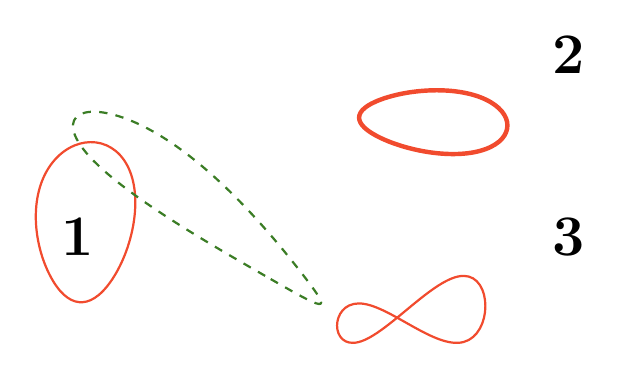
\begin{tikzpicture}[scale=0.7]
% \draw[fill=blue!20] plot [smooth cycle, tension = 0.7] coordinates {(3.4,-1) (3.4, 1) (8.6, 1) (8.6, -1) };
\base
\draw[thick, RedOrange] plot [smooth cycle, tension = 1] coordinates {(-0.4,-0.5) (-0.4, -2.5) (0.7, -2.6) (1, -0.5) };
\node at (0.1,-1.8) {\huge \textbf{1}};
\node at (9,-1.8) {\huge \textbf{3}};
\node at (9,1.5) {\huge \textbf{2}};

\draw[ultra thick, RedOrange] plot [smooth cycle, tension = 1] coordinates {(5.6,0.0) (5.6, 0.7) (7.5, 0.7) (7.5, -0.2) };
\draw[thick, RedOrange] plot [smooth cycle, tension = 1] coordinates {(5.2, -3.7) (5.2,-3) (7.1, -3.7) (7.1, -2.5) };
\draw[thick, OliveGreen, dashed] plot [smooth cycle, tension = 1] coordinates {(4.2, -2.5) (3.5,-2.5)  (0.2, -0.2) (1.5, 0.1) };
\end{tikzpicture}
}

\textit{Figure:} Illustration of one loop of the \textbf{while}
cycle. At the start there are six gray components from previous
loops. The algorithm then computes $\varF$ (red cycles).

Looking at $G ∪ \varF$, we have three components with $\low_1 = 4,
\low_2 = 3, \low_3 = 1$. The component minimizing $\lb(\low(K))$ is the
leftmost one with $\low_1 = 4$ and is set as $\varK$ in Step 6.

Assume there is a light cycle $C$ connecting component $K$ to
to component 3; we add the cycle to $\varX$ and recompute
$\varK$. After recomputation, we have $\low_1 = 1$ and $\low_2 = 3$,
so $\varK$ is set to be component 2.

If there is no light cycle connecting the remaining components, the
\textbf{while} loop terminates with only the thick red cycle being
added to $G$.

\section{Non-constructive: Analysis}

\lem{The while loop of the algorithm terminates in polynomial time and
decreases the number of components.}

\dfn{$X_t ≡$ Contribution from $\varK ∩ \varX$ in the $t$-th step.}

\lem[Bound on $X$]{$w(∑_{t≥1} X_t) ≤ α\cdot \lb(V)$.}

\dfn{$\calF^t ≡ $ set of connected components added from $\varF ∩ \varX$ in the $t$-th step.\par
$\calF^t_i ≡ $ components from $\calF^t$ that touch $P_i$ but not lower parts.
}

\lem[Bound on $F$]{
\begin{itemize}
\item For $H ∈ \calF^t_i$ we have $\lb(H) ≤ \lb(\low(H)) = \lb(P_i)$.
\item We have $\lb(\calF^t_i) ≤ 2 \lb (P_i)$.
\item Finally, $w(⋃_{t} \calF^t) ≤ 2α \cdot \lb(V)$.
\end{itemize}
}

\end{multicols}
\end{document}
